\chapter{ผลการทดลองเบื้องต้นและระบบต้นแบบ}
\label{chapter:results}

บทนี้รายงานผลที่ได้จากการนำระบบที่อธิบายไว้ในบทที่ \ref{chapter:experiment} ไปใช้งานจริงกับวิดีโอที่บันทึกจากพื้นที่ศึกษา โดยแบ่งเนื้อหาออกเป็นสองส่วนตามชื่อบท ส่วนแรกเป็นการแสดงผลการทำงานของระบบต้นแบบในแต่ละโมดูล เพื่อยืนยันว่าองค์ประกอบทั้งสามส่วนทำงานเชื่อมต่อกันได้จริงตั้งแต่ต้นทางจนถึงการแสดงผล ส่วนที่สองเป็นผลการทดลองตามที่ออกแบบไว้ในหัวข้อที่ \ref{sec:experiment-design} ซึ่งประเมินความถูกต้องของผลลัพธ์ในแต่ละขั้นตอนและความหน่วงของการเชื่อมโยงข้อมูล

การนำเสนอเริ่มจากผลการทดลองเบื้องต้นเพื่อคัดเลือกค่าพารามิเตอร์ของขั้นตอนการตรวจจับและติดตามยานพาหนะ ซึ่งเป็นที่มาของค่าที่ระบุไว้ในหัวข้อที่ \ref{subsec:model-params} และ \ref{subsec:tracking} จากนั้นจึงแสดงผลการทำงานของระบบต้นแบบ แล้วตามด้วยผลการทดลองทั้งสี่ชุดเรียงตามลำดับเดียวกับที่ออกแบบไว้ และปิดท้ายด้วยการสรุปเทียบกับเกณฑ์การยอมรับที่กำหนดไว้ล่วงหน้าในตารางที่ \ref{tab:acceptance}

ผลการทดลองทั้งหมดในบทนี้ได้จากการประมวลผลวิดีโอชุดที่ระบุไว้ในตารางที่ \ref{tab:datasets} ด้วยค่าพารามิเตอร์ตามที่กำหนดไว้ในไฟล์ตั้งค่าของแต่ละคลิป โดยบันทึกผลลัพธ์ของแต่ละรอบการประมวลผลแยกจากกัน เพื่อให้สามารถตรวจสอบย้อนกลับได้ว่าตัวเลขแต่ละชุดมาจากการประมวลผลครั้งใด สภาพแวดล้อมที่ใช้ทดสอบประกอบด้วยหน่วยประมวลผล [ระบุ CPU] หน่วยประมวลผลกราฟิก [ระบุ GPU] และหน่วยความจำ [ระบุ RAM] ซึ่งเป็นเครื่องเดียวกันตลอดทุกการทดลอง เพื่อให้ค่าที่เกี่ยวกับความเร็วและความหน่วงเปรียบเทียบกันได้

อนึ่ง ผลที่รายงานในบทนี้เป็นการประเมินระบบต้นแบบภายใต้ชุดข้อมูลและสภาพแวดล้อมที่จำกัด มิใช่การประเมินที่สรุปผลได้ทั่วไปกับถนนทุกเส้นหรือทุกช่วงเวลา ข้อจำกัดของแต่ละการทดลองระบุไว้ท้ายหัวข้อนั้น ๆ และสรุปรวมไว้ในบทที่ \ref{chapter:conclusion}

\section{การทดลองเพื่อเลือกค่าพารามิเตอร์}
\label{sec:param-selection}

ก่อนการทดลองหลักในหัวข้อ 4.3 ถึง 4.6 ผู้วิจัยได้ทดลองเบื้องต้นเพื่อกำหนดพารามิเตอร์สองตัวของโมดูลตรวจจับที่ระบุไว้ในหัวข้อ \ref{subsec:model-params} ได้แก่ ขนาดภาพนำเข้า และค่าขีดแบ่งความเชื่อมั่น การทดลองทั้งสองใช้คลิปเดียวเป็นตัวแทน เพราะวัตถุประสงค์คือเลือกค่าที่เหมาะสมกับมุมกล้องของงานนี้ ไม่ใช่วัดความแม่นยำของระบบ ซึ่งวัดแยกไว้ในหัวข้อ 4.3 ในแต่ละการทดลองปรับพารามิเตอร์เพียงตัวเดียว ส่วนค่าอื่นทั้งหมดคงเดิม และเทียบผลกับค่าจริงที่ผู้วิจัยนับด้วยตาจากคลิปเดียวกัน การทดลองทำตามลำดับ คือเลือกขนาดภาพนำเข้าก่อน แล้วจึงใช้ขนาดภาพที่เลือกได้นั้นในการเลือกค่าขีดแบ่งความเชื่อมั่น ผลการวัดทำบนเครื่องที่มีคุณสมบัติตามที่ระบุไว้ในต้นบทนี้

\subsection{ขนาดภาพนำเข้า}
\label{subsec:exp-imgsz}

กล้องในชุดข้อมูลถูกติดตั้งบนสะพานลอยคนเดินข้าม จึงมองเห็นรถที่อยู่ไกลเป็นวัตถุขนาดเล็กในภาพ ขนาดภาพนำเข้าที่เล็กลงทำให้วัตถุเหล่านี้เหลือพิกเซลน้อยลงก่อนเข้าโมเดล ผู้วิจัยจึงเปรียบเทียบขนาดภาพนำเข้า 3 ค่า ได้แก่ 640, 960 และ 1280 พิกเซล โดยใช้ค่าความเชื่อมั่นและตัวติดตามเดิม วัดจำนวนรถที่นับได้แยกตามชนิดและทิศทาง เทียบกับค่าจริง และวัดอัตราเฟรมต่อวินาทีในการประมวลผล เพราะขนาดภาพที่ใหญ่ขึ้นแลกมาด้วยเวลาประมวลผลที่มากขึ้น

\begin{table}[ht]
\centering
\caption{เปรียบเทียบขนาดภาพนำเข้า}
\label{tab:imgsz}
\begin{tabular}{|c|c|c|c|c|c|c|c|c|c|}
\hline
ขนาดภาพ & \multicolumn{2}{c|}{รถยนต์} & \multicolumn{2}{c|}{มอเตอร์ไซค์} & \multicolumn{2}{c|}{รถบัส} & \multicolumn{2}{c|}{รถบรรทุก} & FPS \\
\cline{2-9}
 & เข้า & ออก & เข้า & ออก & เข้า & ออก & เข้า & ออก & \\
\hline
ค่าจริง & 5 & 14 & 9 & 2 & 0 & 0 & 0 & 0 & -- \\
\hline
640 &19 &14&12 &3 &0 &0 &4 &4 & 14.89\\
\hline
960 & 18 & 14 & 16 & 11 & 0 & 0 & 5 & 6 & 14.99\\
\hline
1280 & 19 & 16 & 17 & 15 & 0 & 0 & 5 & 3 & 12.98 \\
\hline
\end{tabular}
\end{table}

\begin{figure}[ht]
\centering
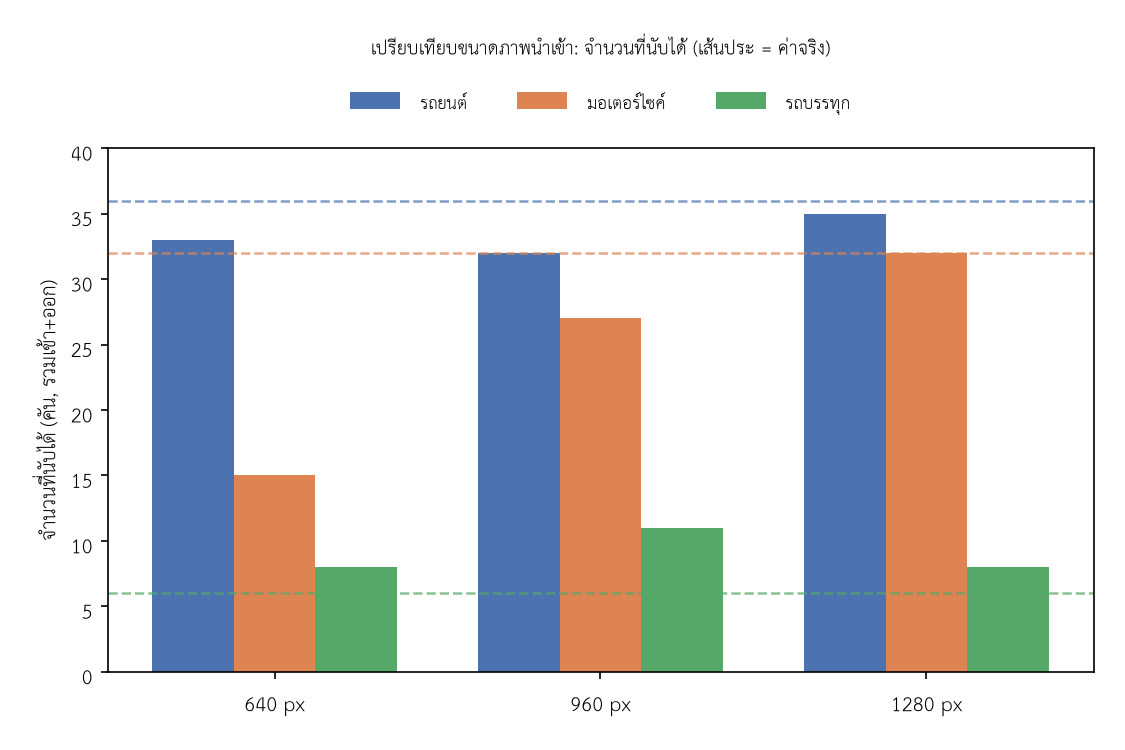
\includegraphics[width=0.85\textwidth]{figures/fig_imgsz_comparison.png}
\caption{เปรียบเทียบจำนวนที่นับได้และความเร็วประมวลผลที่ขนาดภาพนำเข้าต่างกัน เส้นประแสดงค่าจริงของรถยนต์และรถจักรยานยนต์}
\label{fig:imgsz-comparison}
\end{figure}

จากตารางที่ \ref{tab:imgsz} และรูปที่ \ref{fig:imgsz-comparison} ขนาดภาพ 640 พิกเซลนับรถจักรยานยนต์ได้ต่ำกว่าค่าจริงมากที่สุด (12 จาก 2 ทิศทางรวม 11 คัน เทียบกับค่าจริง 11 คัน แต่กระจายผิดทิศทางอย่างเห็นได้ชัด) ขณะที่ขนาด 1280 พิกเซลนับรถจักรยานยนต์ได้ใกล้เคียงค่าจริงที่สุดทั้งสองทิศทาง (17 และ 15 คัน) สอดคล้องกับสมมติฐานว่ารถจักรยานยนต์ซึ่งปรากฏเป็นวัตถุขนาดเล็กในภาพต้องการความละเอียดของภาพนำเข้าที่สูงกว่าจึงจะตรวจจับได้ครบถ้วน ด้านความเร็วประมวลผล ขนาด 640 และ 960 พิกเซลให้อัตราเฟรมใกล้เคียงกัน (14.89 และ 14.99 fps) ขณะที่ 1280 พิกเซลลดลงเหลือ 12.98 fps คิดเป็นการลดลงประมาณร้อยละ 13 ซึ่งถือว่ายอมรับได้เมื่อแลกกับความแม่นยำที่เพิ่มขึ้นอย่างมีนัยสำคัญของรถจักรยานยนต์

ทั้งนี้การเทียบจำนวนรวมอย่างเดียวไม่อาจแยกรถที่ตกหล่นออกจากรถที่นับเกินได้ เพราะสองอย่างนี้อาจหักล้างกัน ตารางนี้จึงใช้เลือกค่าเบื้องต้นเท่านั้น การวัดค่าความแม่นยำ (precision) และค่าการเรียกคืน (recall) อยู่ในหัวข้อ 4.3 ผู้วิจัยจึงเลือกขนาดภาพ \textbf{1280 พิกเซล} เป็นค่ามาตรฐานของระบบ

\subsection{ค่าขีดแบ่งความเชื่อมั่น}
\label{subsubsec:exp-conf}

ค่าขีดแบ่งความเชื่อมั่น (confidence threshold) กำหนดว่าการตรวจจับที่โมเดลให้คะแนนต่ำกว่าค่านี้จะถูกทิ้งตั้งแต่ขั้นตรวจจับ ก่อนจะถึงขั้นติดตามและนับ มอเตอร์ไซค์มีขนาดเล็กและมักบดบังกันในภาพมากกว่ารถยนต์ จึงอาจได้รับคะแนนความเชื่อมั่นต่ำกว่าโดยรวม หากตั้งค่าขีดแบ่งสูงเกินไปอาจตัดมอเตอร์ไซค์ส่วนใหญ่ทิ้งไปตั้งแต่ขั้นตรวจจับ ทำให้การแยกอัตราการไหลของมอเตอร์ไซค์ตามหัวข้อ 3.6.3 ไม่มีข้อมูลให้ใช้ ผู้วิจัยจึงเปรียบเทียบผลการนับที่ค่าขีดแบ่งความเชื่อมั่นสี่ระดับ (0.35, 0.40, 0.50, 0.60) โดยใช้ขนาดภาพนำเข้า 1280 พิกเซลที่เลือกได้ในหัวข้อก่อนหน้า บนคลิป \texttt{traffic-5} ซึ่งเป็นคลิปจราจรปกติที่ใช้เป็นฐานอ้างอิงของระบบ

\begin{table}[ht]
\centering
\caption{ผลการนับที่ค่าขีดแบ่งความเชื่อมั่นต่างกัน}
\label{tab:conf-threshold}
\begin{tabular}{|c|c|c|c|c|}
\hline
ค่าขีดแบ่ง & รถยนต์ & มอเตอร์ไซค์ & รถบรรทุก & รวม \\
\hline
0.35 & 35 & 32 & 8 & 75 \\
\hline
0.40 & 35 & 32 & 8 & 75 \\
\hline
0.50 & 33 & 31 & 7 & 71 \\
\hline
0.60 & 32 & 23 & 8 & 63 \\
\hline
\end{tabular}
\end{table}

\begin{figure}[ht]
\centering
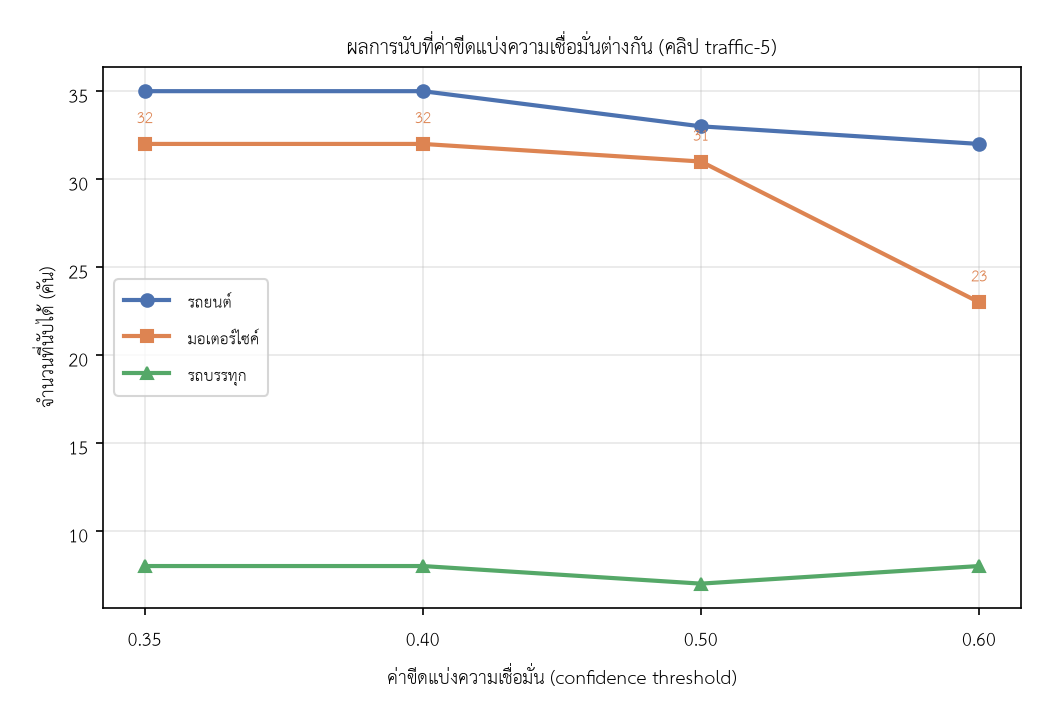
\includegraphics[width=0.78\textwidth]{figures/fig_conf_threshold.png}
\caption{ผลการนับแยกตามชนิดยานพาหนะที่ค่าขีดแบ่งความเชื่อมั่นต่างกัน}
\label{fig:conf-comparison}
\end{figure}

จากตารางที่ \ref{tab:conf-threshold} และรูปที่ \ref{fig:conf-comparison} ค่าขีดแบ่งที่ 0.35 และ 0.40 ให้ผลการนับเท่ากันทุกชนิด แสดงว่าไม่มียานพาหนะคันใดในคลิปนี้ที่ได้คะแนนความเชื่อมั่นอยู่ในช่วงดังกล่าวพอดี เมื่อเพิ่มค่าขีดแบ่งเป็น 0.50 และ 0.60 จำนวนรถจักรยานยนต์ลดลงจาก 32 คันเหลือ 23 คัน คิดเป็นร้อยละ 28 ขณะที่รถยนต์ลดลงจาก 35 คันเหลือ 32 คัน คิดเป็นเพียงร้อยละ 9 และรถบรรทุกแทบไม่เปลี่ยนแปลง (8 คันทั้งที่ค่า 0.35 และ 0.60) รถจักรยานยนต์จึงได้รับผลกระทบจากการเพิ่มค่าขีดแบ่งมากกว่ายานพาหนะประเภทอื่นอย่างไม่สมส่วน สอดคล้องกับสมมติฐานว่าโมเดลให้คะแนนความเชื่อมั่นแก่รถจักรยานยนต์ต่ำกว่ารถยนต์โดยรวม และหากตั้งค่าขีดแบ่งสูงเกินไป สัดส่วนข้อมูลรถจักรยานยนต์ที่สูญหายจะมากกว่ายานพาหนะประเภทอื่นอย่างมีนัยสำคัญ

ผู้วิจัยจึงเลือกค่าขีดแบ่งความเชื่อมั่นที่ \textbf{0.35} เป็นค่ามาตรฐานของระบบ เพื่อคงข้อมูลรถจักรยานยนต์ไว้ให้มากที่สุด ความเสี่ยงด้านผลบวกลวงจากการตั้งค่าต่ำถูกลดทอนด้วยกลไกสองชั้นที่มีอยู่แล้วในระบบ คือการกรองด้วยโซนพื้นที่ (polygon ROI) ตามหัวข้อ 3.3.2 ซึ่งตัดวัตถุนอกบริเวณถนนทิ้งโดยไม่ขึ้นกับค่าความเชื่อมั่น และการโหวตชนิดยานพาหนะข้ามหลายเฟรมตามหัวข้อ 3.5.2 ซึ่งต้องมีผลตรงกันสะสมก่อนจึงจะล็อกชนิดและนับ ไม่ได้ตัดสินจากเฟรมเดียว

\section{ผลต้นแบบของระบบ}
\label{sec:prototype-results}

หัวข้อนี้แสดงผลการทำงานของระบบต้นแบบในแต่ละขั้นของสายท่อข้อมูล ตั้งแต่การตรวจจับยานพาหนะไปจนถึงการแสดงผลบนแฝดดิจิทัล เพื่อยืนยันว่าทั้งสามโมดูล (AI Worker, Backend, Unity) เชื่อมต่อและทำงานร่วมกันได้จริง พร้อมแสดงหลักฐานที่เป็นรูปธรรมของแต่ละขั้นตอน ส่วนความแม่นยำและตัวชี้วัดเชิงปริมาณของแต่ละส่วนแสดงแยกไว้ในหัวข้อ 4.3 ถึง 4.6

\subsection{การกำหนดพื้นที่ตรวจวัดและการตรวจจับยานพาหนะ}
\label{subsec:proto-detection}

AI Worker ประมวลผลจากไฟล์วิดีโอที่บันทึกไว้ล่วงหน้า ไม่ใช่สัญญาณสดจากกล้องวงจรปิด เนื่องจากยังไม่ได้รับสิทธิ์เข้าถึงกล้อง CCTV ของสถาบันในช่วงที่พัฒนา ระบบใช้ YOLOv8s ร่วมกับ ByteTrack ตามที่อธิบายไว้ในหัวข้อ \ref{subsec:model-params} และ \ref{subsec:tracking} ตรวจจับและติดตามยานพาหนะ 4 ชนิด (รถยนต์ มอเตอร์ไซค์ รถบัส รถบรรทุก)

ก่อนรันการตรวจจับ ผู้วิจัยกำหนดพื้นที่ตรวจวัด (polygon) เส้นนับ (counting line) และพื้นที่วัดความหนาแน่น (occupancy polygon) ของแต่ละมุมกล้องด้วยเครื่องมือคลิกพิกัดจากเฟรมจริงของวิดีโอ ดังตัวอย่างในรูปที่ \ref{fig:zone-calibration} ซึ่งแสดงการวาดโซนทับบนภาพจริงจากกล้องที่ติดตั้งบนสะพานลอยถนนฉลองกรุง สถาบันเทคโนโลยีพระจอมเกล้าเจ้าคุณทหารลาดกระบัง โซนสีเหลือง (\texttt{in}) และสีฟ้า (\texttt{out}) ครอบคลุมช่องจราจรแต่ละฝั่ง ส่วนเส้นสีแดงคือเส้นนับที่ใช้ตัดสินว่ายานพาหนะข้ามผ่านแล้วหรือยัง

\begin{figure}[ht]
\centering
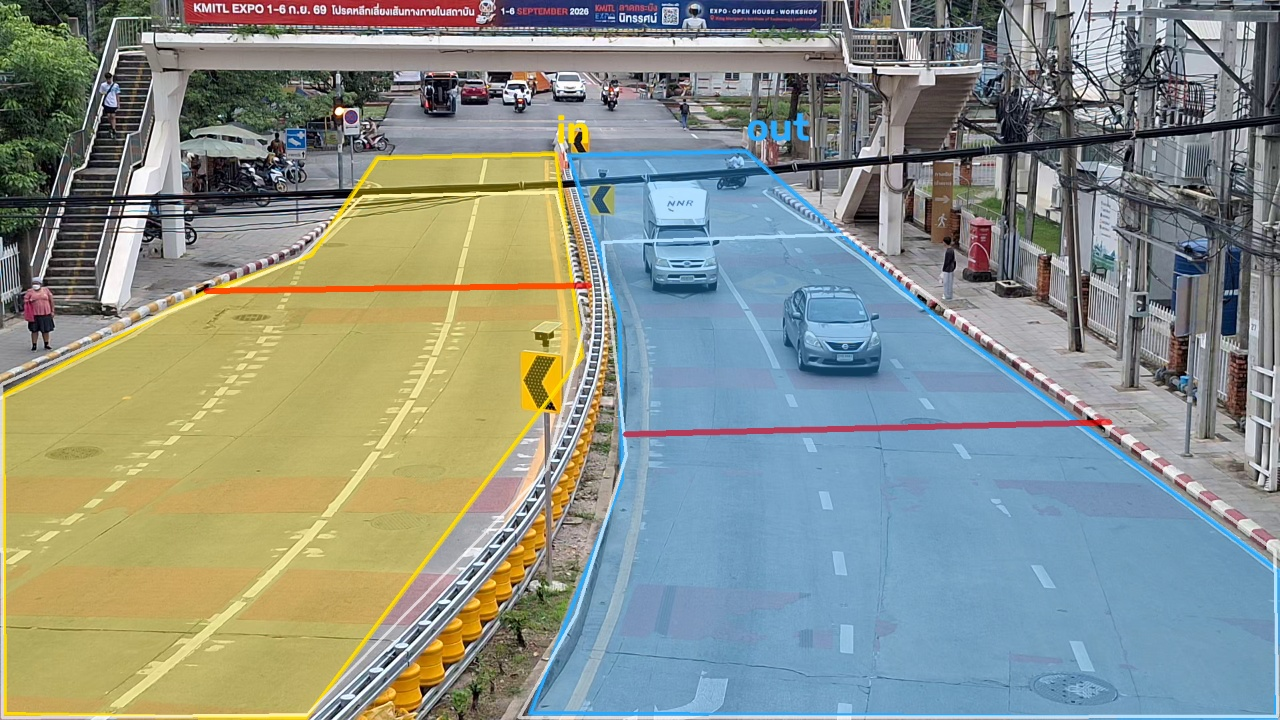
\includegraphics[width=\textwidth]{figures/fig_zone_calibration.jpg}
\caption{พื้นที่ตรวจวัดและเส้นนับที่กำหนดไว้บนภาพจริงจากกล้องถนนฉลองกรุง (คลิป \texttt{event-2}) โซนสีเหลืองคือทิศทางเข้า โซนสีฟ้าคือทิศทางออก เส้นสีแดงคือเส้นนับ}
\label{fig:zone-calibration}
\end{figure}

นับยานพาหนะที่ข้ามเส้นตรวจวัดในแต่ละโซนตามกลไกในหัวข้อ \ref{sec:counting} ทดสอบกับคลิปจริงหลายคลิปจากมุมกล้องต่างกันตามที่ระบุไว้ในหัวข้อ \ref{sec:data-collection} ผลลัพธ์ของแต่ละการรันถูกบันทึกเป็นไฟล์ (เหตุการณ์การนับ อัตราการครอบครองพื้นที่ และคำตัดสินสภาพการจราจรรายหน้าต่างเวลา) ซึ่งนำไปใช้ในการทดลองหัวข้อ 4.3 ถึง 4.5 ต่อไป

ระบบวัดความเร็วในการประมวลผลจริงได้ด้วย (ไม่นับเวลาที่หยุดดูภาพค้างไว้) ตัวอย่างจากคลิป \texttt{event-1} วัดได้ 21.19 เฟรมต่อวินาที เทียบกับอัตราเฟรมของวิดีโอต้นฉบับที่ 25.00 เฟรมต่อวินาที แสดงว่าเครื่องมือทดสอบประมวลผลได้ช้ากว่าความเร็วของวิดีโอต้นฉบับเล็กน้อย ตัวเลขชุดนี้เป็นเพียงตัวอย่างยืนยันว่าเครื่องมือวัดทำงานได้ ส่วนผลเปรียบเทียบตามขนาดภาพนำเข้าอยู่ในตารางที่ \ref{tab:imgsz}

\subsection{การตรวจสอบและส่งต่อข้อมูล}
\label{subsec:proto-backend}

Backend (Node.js, Express, Socket.IO) รับข้อมูลเหตุการณ์การนับจาก AI Worker ผ่าน HTTP POST ตรวจสอบรูปแบบข้อมูลตามสัญญาข้อมูลที่กำหนดไว้ (ชนิดรถ ทิศทาง ค่าความเชื่อมั่น ต้องอยู่ในรูปแบบที่ถูกต้อง) ข้อมูลที่ไม่ถูกต้องจะถูกปฏิเสธพร้อมเหตุผล ข้อมูลที่ผ่านการตรวจสอบจะถูกเก็บสะสมเป็นตัวนับแยกตามชนิดและทิศทาง แล้วกระจายต่อผ่าน Socket.IO ตามที่อธิบายไว้ในหัวข้อ \ref{sec:realtime-delivery} สองช่องทางหลัก คือช่องทาง \texttt{spawn} สำหรับแดชบอร์ดของผู้พัฒนา และช่องทาง \texttt{spawn\_vehicle} ที่ตัดข้อมูลให้เหลือเฉพาะฟิลด์ที่จำเป็นสำหรับส่งต่อให้ Unity

ผู้วิจัยยืนยันการทำงานครบวงจรด้วยการเล่นข้อมูลจากคลิปจริงซ้ำเข้าสู่ Backend ที่รันอยู่จริง ข้อมูลทุกรายการถูกส่งและได้รับสำเร็จโดยไม่มีรายการถูกปฏิเสธผิดพลาด ดังแสดงในรูปที่ \ref{fig:dashboard-overview} ซึ่งเป็นหน้าแดชบอร์ดสำหรับผู้พัฒนาขณะรับข้อมูลจากคลิป \texttt{event-2} แสดงยอดนับสะสม 100 คัน แยกเป็นทิศทางเข้า 53 คันและออก 47 คัน พร้อมแยกย่อยตามชนิดยานพาหนะ

\begin{figure}[ht]
\centering
% \includegraphics[width=0.85\textwidth]{figures/fig_dashboard_overview.png}
\caption{หน้าแดชบอร์ดของ Backend ขณะรับข้อมูลจริงจากคลิป \texttt{event-2} — ยอดนับสะสม 100 คัน แยกทิศทางเข้า 53 คัน ออก 47 คัน และแยกตามชนิดยานพาหนะ}
\label{fig:dashboard-overview}
\end{figure}
% TODO: เปิด http://localhost:3000 ขณะรัน `python -m src.replay --from runs/event-2_slow-moving --backend`
% แล้ว screenshot หน้าจอ บันทึกเป็น docs/figures/fig_dashboard_overview.png แล้วลบบรรทัด % ด้านบน

\subsection{การแสดงผลบนแฝดดิจิทัลสามมิติ}
\label{subsec:proto-unity}

ส่วนแสดงผลพัฒนาด้วย Unity เวอร์ชัน 6000.4.1f1 เชื่อมต่อกับ Backend ผ่าน Socket.IO ตามสถาปัตยกรรมในหัวข้อ \ref{sec:visualization} และรับข้อมูลสองช่องทาง คือเหตุการณ์การข้ามเส้นของยานพาหนะแต่ละคัน (\texttt{spawn\_vehicle}) และคำตัดสินสภาพการจราจรรายโซน (\texttt{traffic\_state}) เมื่อได้รับเหตุการณ์ยานพาหนะ ระบบจะดึงแบบจำลองสามมิติจากกลุ่มวัตถุที่เตรียมไว้ (ไม่ได้สร้างจำนวนคงที่ไว้ล่วงหน้า แต่สร้างเมื่อต้องใช้จริง) มาวางตำแหน่งและให้เคลื่อนที่ตามเส้นทางที่กำหนด เมื่อได้รับคำตัดสินสภาพการจราจรของแต่ละโซน ระบบจะปรับช่วงความเร็วของยานพาหนะที่สปอนในโซนนั้นให้สอดคล้องกับสภาพที่ตัดสินได้ เช่น โซนที่สภาพเป็นรถติดสนิทหรือหนาแน่นสูง ความเร็วของยานพาหนะที่แสดงจะช้าลงกว่าช่วงปกติ ทดสอบเชื่อมต่อครบทั้งสองช่องทางแล้ว ระบบแสดงทั้งตำแหน่งยานพาหนะและสถานะการจราจรได้ถูกต้อง ดังแสดงในรูปที่ \ref{fig:unity-live}

\begin{figure}[ht]
\centering
% \includegraphics[width=0.8\textwidth]{figures/fig_unity_live.png}
\caption{การแสดงผลบน Unity ขณะรับข้อมูลยานพาหนะและสถานะการจราจรจากคลิปจริง}
\label{fig:unity-live}
\end{figure}

\section{ความแม่นยำของการนับยานพาหนะ}
\label{sec:res-counting}

การทดลองนี้ตามที่ออกแบบไว้ในหัวข้อ \ref{subsec:exp-accuracy} เปรียบเทียบจำนวนยานพาหนะที่ระบบนับได้กับค่าจริงที่นับด้วยตาจากคลิปวิดีโอ 5 คลิปจากมุมกล้องเดียวกัน ([ระบุชื่อ 5 คลิป] ดูรายละเอียดชุดข้อมูลในตารางที่ \ref{tab:datasets}) การนับด้วยตาทำก่อนดูผลของระบบเพื่อไม่ให้ลำเอียง แยกนับตามชนิดยานพาหนะและทิศทาง รายงานผลทั้งแบบแยกรายคลิปและแบบรวมทุกคลิป โดยใช้ขนาดภาพนำเข้าและค่าขีดแบ่งความเชื่อมั่นที่เลือกได้จากหัวข้อ \ref{sec:param-selection} (1280 พิกเซล และ 0.35 ตามลำดับ)

\begin{table}[ht]
\centering
\caption{ผลการนับยานพาหนะแยกรายคลิป}
\label{tab:exp1-perclip}
\begin{tabular}{|c|c|c|c|c|}
\hline
คลิป & ค่าจริง (คัน) & นับได้ (คัน) & Precision & Recall \\
\hline
traffic-1 & [ระบุ] & 30 & [ระบุ] & [ระบุ] \\
\hline
traffic-2 & [ระบุ] & 74 & [ระบุ] & [ระบุ] \\
\hline
traffic-4 & [ระบุ] & 19 & [ระบุ] & [ระบุ] \\
\hline
traffic-5 & [ระบุ] & 75 & [ระบุ] & [ระบุ] \\
\hline
traffic-6 & [ระบุ] & 62 & [ระบุ] & [ระบุ] \\
\hline
\end{tabular}
\end{table}

\begin{table}[ht]
\centering
\caption{ผลรวมทุกคลิป แยกตามชนิดยานพาหนะ}
\label{tab:exp1-pooled}
\begin{tabular}{|l|c|c|c|c|c|c|c|c|}
\hline
ชนิด & ค่าจริง & นับได้ (TP) & FP & FN & Precision & Recall & F1-score & MAE \\
\hline
รถยนต์ & & & & & & & & \\
\hline
มอเตอร์ไซค์ & & & & & & & & \\
\hline
รถบัส/รถบรรทุก & & & & & & & & \\
\hline
\textbf{รวม} & & & & & & & & \\
\hline
\end{tabular}
\end{table}

จากตารางที่ \ref{tab:exp1-perclip} และ \ref{tab:exp1-pooled} [สรุปว่าชนิดไหนแม่นกว่า และเทียบกับเกณฑ์การยอมรับในตารางที่ \ref{tab:acceptance} ว่าผ่านหรือไม่ — เขียนได้หลังกรอกคอลัมน์ "ค่าจริง" จากการนับมือครบทั้ง 5 คลิป]

\section{ความแม่นยำของการจำแนกสภาพจราจร}
\label{sec:res-classification}

การทดลองนี้ตามที่ออกแบบไว้ในหัวข้อ \ref{subsec:exp-classification} เปรียบเทียบสถานะที่ระบบตัดสินในแต่ละหน้าต่างเวลา 20 วินาที กับสถานะจริงที่กำกับไว้จากการดูวิดีโอ เนื่องจากระบบตัดสินสถานะแยกรายโซน (ฝั่งเข้าและฝั่งออก) ไม่ใช่ค่าเดียวทั้งคลิป การกำกับค่าจริงจึงทำแยกโซนด้วยเช่นกัน ไม่ใช่กำกับภาพรวมคลิปเดียว ผู้วิจัยใช้คลิป \texttt{event-2} ซึ่งเป็นคลิปเดียวที่เกณฑ์ตัดสิน (ตารางที่ \ref{tab:traffic-state-rules}) สอบเทียบด้วยหลักฐานเชิงประจักษ์แล้ว ได้ข้อมูลทั้งหมด 10 หน้าต่างเวลา คูณ 2 โซน รวม 20 ค่า

\begin{table}[ht]
\centering
\caption{Confusion Matrix การจำแนก 4 สถานะ (รวมทุกโซนทุกคลิป)}
\label{tab:confusion}
\begin{tabular}{|l|c|c|c|c|}
\hline
สภาพจริง $\backslash$ ผลประเมิน & Normal & High Density & Slow Moving & Standstill \\
\hline
Normal & 15 & 0 & 1 & 0 \\
\hline
High Density & 0 & 0 & 0 & 0 \\
\hline
Slow Moving & 0 & 0 & 0 & 1 \\
\hline
Standstill & 0 & 0 & 1 & 2 \\
\hline
\end{tabular}
\end{table}

ความถูกต้องโดยรวม (Overall Accuracy) เท่ากับ 0.85 จากทั้งหมด 20 ค่า (10 หน้าต่างเวลา $\times$ 2 โซน) ซึ่งสูงกว่าเกณฑ์การยอมรับที่กำหนดไว้ ($\geq 0.70$)

จากตารางที่ \ref{tab:confusion} ที่สำคัญที่สุดคือต้องตรวจสอบว่าไม่มีกรณีที่สถานะจริงเป็น Standstill แต่ระบบตัดสินเป็น Normal เพราะเป็นเกณฑ์การยอมรับขั้นเด็ดขาดตามตารางที่ \ref{tab:acceptance} (ถ้ามีแม้แต่ 1 กรณี ต้องรายงานตรง ๆ ว่าไม่ผ่านเกณฑ์นี้) จากข้อมูลที่เก็บได้ไม่พบกรณีดังกล่าวเลย (0 กรณี) ระบบจึงผ่านเกณฑ์ขั้นเด็ดขาดนี้ ข้อผิดพลาดทั้งสามกรณีที่พบเกิดขึ้นเฉพาะระหว่างสถานะ Slow Moving กับ Standstill ซึ่งเป็นสองสถานะที่อยู่ติดกันตามระดับความรุนแรง ไม่มีกรณีที่คลาดเคลื่อนข้ามไปถึงสถานะ Normal หรือ High Density แสดงว่าความผิดพลาดของระบบเป็นความคลาดเคลื่อนเล็กน้อยระหว่างระดับใกล้เคียงกัน ไม่ใช่การตัดสินผิดพลาดแบบสุ่ม

ข้อจำกัดที่พบคือสถานะ High Density ไม่ปรากฏในข้อมูลที่ทดสอบเลย เนื่องจากคลิป \texttt{event-2} ไม่มีช่วงเวลาที่การจราจรหนาแน่นแต่ยังไหลได้ดีเกิดขึ้นจริง จึงไม่สามารถประเมินค่า Recall ของสถานะนี้ได้ ต้องถือเป็นช่องว่างของชุดข้อมูลทดสอบ มิใช่ตัวเลขที่มีความหมายทางสถิติ

\section{ผลของการแยกอัตราการไหลของรถจักรยานยนต์}
\label{sec:res-separation}

การทดลองนี้ตามที่ออกแบบไว้ในหัวข้อ 3.9.3 เปรียบเทียบผลการจำแนกสภาพจราจรระหว่างแบบที่นับอัตราการไหลรวมทุกชนิด กับแบบที่แยกอัตราการไหลของรถยนต์ออกจากรถจักรยานยนต์ตามที่ออกแบบไว้ในหัวข้อ 3.6.3 ผู้วิจัยพบกรณีตัวอย่างที่แสดงปัญหานี้ชัดเจนจากคลิป \texttt{event-2} ช่วงเวลา 160 ถึง 180 วินาที โซนทิศทางเข้า ดังตารางที่ \ref{tab:motorcycle-separation}

\begin{table}[ht]
\centering
\caption{เปรียบเทียบผลการตัดสินระหว่างวิธีนับรวมกับวิธีแยกอัตราการไหล}
\label{tab:motorcycle-separation}
\begin{tabular}{|l|c|}
\hline
\textbf{ตัวแปร} & \textbf{ค่าที่วัดได้} \\
\hline
ความหนาแน่น (O) & 9.54 คันต่อเฟรม \\
\hline
อัตราการไหลรถยนต์ ($V_c$) & 6.0 คันต่อนาที (2 คัน) \\
\hline
อัตราการไหลรถจักรยานยนต์ ($V_{mc}$) & 18.0 คันต่อนาที (6 คัน) \\
\hline
ผลตัดสินแบบนับรวม ($V_c+V_{mc}=24.0$) & \textbf{Slow Moving} \\
\hline
ผลตัดสินแบบแยก (ใช้ $V_c$ เท่านั้น) & \textbf{Standstill} \\
\hline
\end{tabular}
\end{table}

ในช่วงเวลานี้รถยนต์เคลื่อนผ่านเส้นนับได้เพียง 2 คันใน 20 วินาที ขณะที่รถจักรยานยนต์เคลื่อนผ่านได้ถึง 6 คัน หากนับอัตราการไหลรวมกันตามวิธีดั้งเดิม ความเคลื่อนไหวของรถจักรยานยนต์จะบดบังสัญญาณรถติด ทำให้ระบบตัดสินว่าการจราจรเคลื่อนตัวได้ (Slow Moving) ทั้งที่รถยนต์แทบไม่ขยับ การแยกอัตราการไหลตามที่ออกแบบไว้แก้ปัญหานี้โดยตรง โดยตัดสินได้อย่างถูกต้องว่าอยู่ในสภาวะหยุดนิ่ง (Standstill) สอดคล้องกับเกณฑ์การยอมรับที่กำหนดว่าต้องมีหน้าต่างเวลาอย่างน้อย 1 หน้าต่างที่คำตัดสินเปลี่ยนแปลงอย่างมีนัยสำคัญ

\section{ความหน่วงของการเชื่อมโยงข้อมูล}
\label{sec:res-latency}

การทดลองนี้ตามที่ออกแบบไว้ในหัวข้อ \ref{subsec:exp-latency} วัดเวลาที่ข้อมูลใช้เดินทางจากจุดที่ AI Worker ตรวจพบเหตุการณ์การข้ามเส้น ไปจนถึงจุดที่ Unity แสดงยานพาหนะนั้นบนหน้าจอ แบ่งเป็น 4 ช่วง

\begin{table}[ht]
\centering
\caption{ความหน่วงแบ่งตามช่วงการส่งผ่านข้อมูล}
\label{tab:latency}
\begin{tabular}{|l|c|c|}
\hline
ช่วงการส่งผ่านข้อมูล & Median (ms) & P95 (ms) \\
\hline
1. AI Worker ประมวลผลและสร้างเหตุการณ์ & & \\
\hline
2. ส่ง HTTP POST ถึงการตรวจสอบของ Backend & & \\
\hline
3. Backend กระจายผ่าน WebSocket & & \\
\hline
4. Unity รับและสปอนยานพาหนะ & & \\
\hline
\textbf{รวมความหน่วงปลายทางถึงปลายทาง} & \textbf{} & \textbf{} \\
\hline
\end{tabular}
\end{table}

[ย่อหน้าวิเคราะห์ผล — เขียนได้หลังมีข้อมูลจริงเท่านั้น เทียบกับเกณฑ์การยอมรับ (ความหน่วงมัธยฐานไม่เกิน 1 วินาที) ในตารางที่ \ref{tab:acceptance} หากยังไม่สามารถวัดได้ครบทั้ง 4 ช่วง ให้ระบุตรง ๆ ว่าวัดได้ถึงช่วงใด และเหตุใดช่วงที่เหลือจึงยังวัดไม่ได้]
